\addchap{Programming guide}

\chapter{\icewing{} Files} 

\section{Filesystem hierarchy}
\label{sec:p_filesystem}

Let's see, what the installation consists of. Below the
installation prefix, for example ``/usr/local'', you have this
structure-content:
\begin{description}
\item[bin]
  \begin{description}
  \item icewing (the executable itself)
  \item icewing-config

    A shell script similar to e.g. gtk-config which makes compiling
    of own plugins easy. It generates compiler-flags, extracts
    system-paths and more.
  \end{description} 
\item [include] - All the headers for your own plugin programming
  \begin{description}
  \item iceWing - headers from the \icewing{} system
  \item iwPlugins - plugin headers

    If your plugin pubishes new structures to be used by other
    plugins, you probably want to put them here.
  \end{description}
\item [lib/iceWing]
  Here is the default place for \icewing{} to search for plugin
  libraries. Normally you give \icewing{} by command line parameter
  ``-l'' library names to load. If \icewing{} is not able to load
  them, it automatically tries to load them from this directory.
\item [man] - The manpage of \icewing{}
\item [share]
  \begin{description}
  \item iceWing - Place where plugins can store additional data
    files.

    E.g. the plugin ``Face'' has here it's config-file placed, and
    the polynom-classificator plugin stores it's data here, too.
  \item log/icewing.log - the installation log file
  \end{description}
\end{description} 

%######################
\section{Headerfiles overview}
\label{sec:headerfiles}

TODO

%\chapter{General structure of a plugin}
%\section{Sources}
%\subsection{plugins/min/min.c}
%\subsection{plugins/min/min.cpp (Brief discussion: C vs C++)}
%\section{Compiling}
%First cd into the source-path of that plugin, check/edit the
%Makefile for e.g. correct ``FLAGS'' entry. Then compile the library
%with this commands:
%\sS
%\shellcom{make depend}
%\shellcom{make}
%\subsection{icewing-config}
%\subsection{Makefile for the ``typical plugin''}
%
%\chapter{Gui}
%\section{The available widgets \label{sec:widgetProgramming}}
%\section{How to Display own plugin results}
%\section{How to load|save|create images|video streams}
%
%\chapter{How plugins communicate}
%\section{How to put/get own data}
%\section{The ``observer'' interface}
%\section{The funktions interface}
%\section{Data source|sink plugins}
%
%\chapter{\icewing{} and C vs C++, more verbose}
%
%\chapter{The small toolbox ``tools.h'' }
%\section{Messages}
%\section{How to use ``timestamps''}

\selectlanguage{german}

\chapter{\icewing{} -- Ein CASE Tool}

\begin{center}
  \vspace{-0.5cm}
  \Large \textbf{Currently only available in German.}
  \vspace{0.1cm}
\end{center}

\begin{quote}
  \textbf{Originally taken from \cite[Anhang B]{Loemker2004-LVO}.
  Since then updated according to changes in \icewing{}}
\end{quote}

\index{iceWing}
\label{chap:p_icewing}

Bei der Entwicklung von Software im wissenschaftlichen Bereich gibt
es einige sehr aufwendige Aufgaben, die jedes mal wieder anfallen,
aber nicht direkt zu der eigentlichen Aufgabe geh"oren. Sehr h"aufig
ben"otigt man eine M"oglichkeit, m"oglichst einfach und schnell
Parameter eines Algorithmus zu beeinflussen. "Ahnlich wichtig ist
auch die M"oglichkeit der einfachen visuellen Darstellung von
beliebigen Daten. Die Daten m"ussen jederzeit
leicht inspizierbar und abspeicherbar sein. Bei gr"o"seren
integrierten Systemen ist es von Vorteil, wenn Einzelkomponenten
getrennt voneinander entwickelt werden k"onnen und anschlie"send mit
m"oglichst wenig Geschwindigkeitsverlust untereinander flexibel
kommunizieren k"onnen.

Eine ergonomisch ausgefeilte Oberfl"ache, die auch f"ur mit einem
Programm nicht vertraute Person leicht bedienbar ist, wird im
wissenschaftlichen Bereich dagegen meist nicht ben"otigt. Wichtig
ist meist, da"s ein kleines mit der zu l"osenden Aufgabe gut
vertrautes Team einfach ihren speziellen Algorithmus entwickeln und
optimieren kann. Dieses Team von Spezialisten mu"s die Oberfl"ache
leicht bedienen k"onnen. Dabei soll meist kein fertiges Programm
f"ur einen Endanwender entstehen. Verschiedene Systeme bieten auf
diesen Gebieten schon Funktionalit"at an. Das kommerzielle
\matlab{}\index{Matlab} hat beispielsweise umfangreiche
M"oglichkeiten zur Visualisierung und zur Oberfl"achengenerierung,
die durch die \matlab{} eigene Scriptsprache einfach benutzt werden
k"onnen \cite{Matlab2003}. Die freie Scriptsprache Tcl mit ihrem
graphischen Toolkit Tk\index{Tcl/Tk} bietet ebenfalls sehr einfache
M"oglichkeiten, eine Oberfl"ache zu generieren
\cite{Ousterhout1994-TAT}.

Bestehende Systeme sind allerdings meist nicht auf die speziellen
Belange bei der Entwicklung von wissenschaftlicher Software
optimiert. Daher wurde \icewing{}, \emph{the Integrated
Communication Environment Which Is Not Gesten}\footnote{Dies ist
ein Hinweis auf ein "alteres Programm, den Vorg"anger von
\icewing{}.}, neu entwickelt. \icewing{} ist eine graphische Shell,
die f"ur zur Laufzeit nachladbare Plugins\index{Plugin} die oben
angef"uhrten Funktionalit"aten auf einfache Weise zur Verf"ugung
stellt. In den n"achsten Abschnitten wird \icewing{} nun n"aher
vorgestellt. Dazu wird zuerst ein "Uberblick "uber die Erstellung
von Plugins gegeben. Die nachfolgenden Kapitel gehen dann auf
verschiedene Details exemplarisch n"aher ein. Somit ist die folgende
Beschreibung kein komplettes Referenzhandbuch mit einer Darstellung
aller Funktionen und Typen von \icewing{}. Weitere hier nicht
erw"ahnte Punkte finden sich in den Headern und den Beispielplugins
von \icewing{}.

\section{"Uberblick}

\begin{figure}[htb]
  \begin{center}
    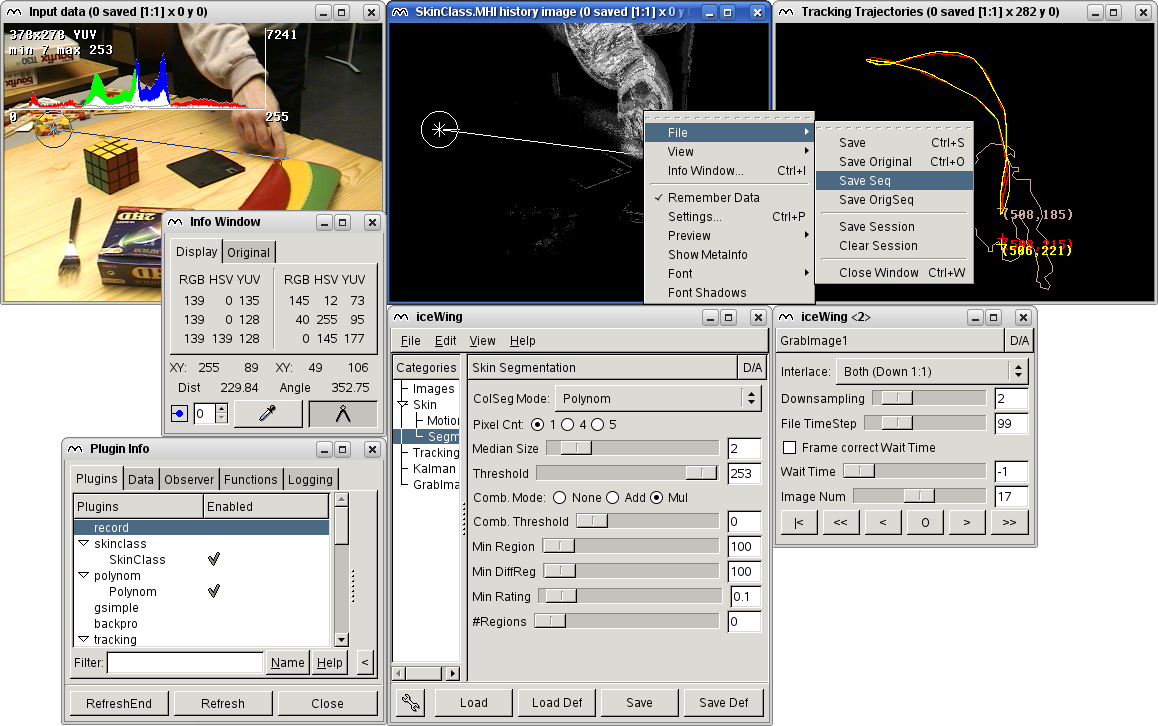
\includegraphics[width=\textwidth]{iw_main}
  \end{center}
  \caption[Eine typische Sitzung mit \icewing{}]
  {Eine typische Sitzung mit \icewing{}. Verschiedene
    Zwischenergebnisse sind visualisiert und k"onnen begutachtet
    werden. Auf verschiedene Parameter kann interaktiv Einflu"s
    genommen werden.}
  \label{fig:p_icewing}
\end{figure}

\icewing{} ist ein in C geschriebenes Programm, das als shared
Libraries \index{shared Library} realisierte Plugins zur Laufzeit
nachladen kann. Getestet wurde es unter i386 Linux mit dem GCC
Version 2.95 bis Version 4.0\footnote{siehe http://gcc.gnu.org/} und
auf Alphas unter OSF 4.0f mit den Compilern DEC~C Version 5.9 und
GCC Version 3.1. F"ur graphische Ausgaben und die
Oberfl"achengenerierung wird zwingend das \Index{GTK}
Toolkit\footnote{siehe http://www.gtk.org/} in der Version~1.2
ben"otigt. Durch andere externe Libraries kann der Funktionsumfang
beispielsweise bez"uglich unterst"utzter Graphikformate gesteigert
werden. Abbildung~\ref{fig:p_icewing} zeigt eine typische Sitzung
mit \icewing{}, bei der H"ande in einer Bildsequenz segmentiert und
verfolgt werden.

\paragraph{Plugins in \icewing{}}\hfill\\

Das Hauptprogramm \icewing{} stellt nur eine initiale Oberfl"ache
und verschiedene Hilfsroutinen zur Verf"ugung. Die eigentliche
Funktionalit"at wird durch Plugins realisiert. Plugins f"ur
\icewing{} m"ussen das in Abbildung~\ref{fig:p_plugdef}
dargestellte Interface implementieren. An Hand eines minimalen
Plugins ist dies in Abbildung~\ref{fig:p_min} dargestellt. Wird ein
Plugin in Form einer shared Library geladen, wird zuerst eine
Funktion mit Namen \fktIndex{plug$\_$get$\_$info()} aufgerufen. Dies
ist zugleich der einzig fest vorgegebene Einsprungpunkt in die
Library. Die Funktion dient der Instantiierung einer neuen Instanz
eines Plugins, sie hat damit die Aufgabe einer
\Index{Factory-Funktion}. Die Funktion gibt einen Zeiger auf eine
gef"ullte Struktur vom Typ \typeIndex{plugDefinition} zur"uck.

\begin{figure}[htb]
  \begin{center}
    \begin{small}
      \ovalbox{%
      \linespread{0.9}
\begin{BVerbatim}
typedef struct plugDefinition {
    char *name;
    plugType type;
    void (*init) (struct plugDefinition *plug,
                  grabParameter *para, int argc, char **argv);
    int  (*init_options) (struct plugDefinition *plug);
    void (*cleanup) (struct plugDefinition *plug);
    BOOL (*process) (struct plugDefinition *plug,
                     char *id, struct plugData *data);
} plugDefinition;
\end{BVerbatim}%
      }
    \end{small}
  \end{center}
  \caption[Die Struktur plugDefinition]
  {Die Struktur plugDefinition, die Plugins implementieren m"ussen.}
  \label{fig:p_plugdef}
\end{figure}

Die Struktur \type{plugDefinition} enth"alt alle Informationen, die
\icewing{} "uber ein neues Plugin haben mu"s. Die Funktionszeiger
\fkt{init()}, \fkt{init\_options()}, \fkt{cleanup()} und
\fkt{process()} definieren Einsprungpunkte f"ur die Instanz des
Plugins. \fkt{init()} dient der allgemeinen Initialisierung einer
Instanz. Hier werden beispielsweise auch Kommandozeilenargumente
verarbeitet. In \fkt{init\_options()} wird das graphische
Benutzerinterface initialisiert. Genaueres hierzu findet sich in
Abschnitt~\ref{sec:p_gui}. \fkt{cleanup()} wird am Programmende
aufgerufen, um die Freigabe von Ressourcen zu
erm"oglichen. \fkt{process()} wird schlie"slich aufgerufen, wenn die
eigentliche Funktionalit"at des Plugins ausgef"uhrt werden
soll. Wann dies der Fall ist, kann mit Hilfe der Funktionen zur
Kommunikation zwischen Plugins definiert werden. N"aheres hierzu
findet sich in Abschnitt~\ref{sec:p_kommunikation}. Die Variable
\var{name} gibt den Namen der Instanz an. Da der Name zur
Identifikation der Instanz dient, mu"s er eindeutig sein. \var{type}
sollte aus Kompatibilit"atsgr"unden immer auf \var{PLUG\_IMAGE}
gesetzt werden.

\begin{figure}[htb]
  \begin{center}
    \begin{small}
      \ovalbox{%
      \linespread{0.9}
\begin{BVerbatim}
#include "main/plugin.h"

static void min_init (plugDefinition *plug,
                      grabParameter *para, int argc, char **argv)
{
    ...
}

...

static plugDefinition plug_min = {
    "Min",
    PLUG_IMAGE,
    min_init,
    min_init_options,
    min_cleanup,
    min_process
};

plugDefinition *plug_get_info (int cnt, BOOL *append)
{
    *append = TRUE;
    return &plug_min;
}
\end{BVerbatim}%
      }
    \end{small}
  \end{center}
  \caption[Ein minimales Plugin]
  {Das Grundger"ust eines minimalen Plugins.}
  \label{fig:p_min}
\end{figure}

Da das Plugin aus Abbildung~\ref{fig:p_min} immer einen festen
Namen zur"uckgibt, l"a"st es sich nur einmal instantiieren. Um dies
zu "andern, mu"s die Struktur vom Typ \type{plugDefinition}
dynamisch alloziert werden und der dort enthaltene Name mu"s
eindeutig gemacht werden. Dies kann durch die Integration der
Instanznummer \var{cnt} in den Namen geschehen. \var{cnt} gibt an,
wie h"aufig das Plugin schon instantiiert werden
sollte. \fkt{plug\_get\_info()} "andert sich damit zu:
\begin{small}
\linespread{0.9}
\begin{verbatim}
    *append = TRUE;
    plugDefinition *def = calloc (1, sizeof(plugDefinition));
    *def = plug_min;
    def->name = g_strdup_printf ("Min%d", cnt);
    return def;
\end{verbatim}
\end{small}
Damit kann das Plugin nun beliebig h"aufig instantiiert werden.

Sollen Plugins in C++ geschrieben werden, kann dies entsprechend dem
bisher erl"auterten Vorgehen geschehen. Alternativ steht aber auch
die in Abbildung~\ref{fig:p_cpp} dargestellte C++-Klasse zur
Verf"ugung. Durch Ableiten von dieser Klasse ist ebenfalls die
Erzeugung einer Plugin-Instanz m"oglich. Die Factory-Funktion
\fkt{plug\_get\_info()} wird in diesem Fall zu
\begin{small}
\linespread{0.9}
\begin{verbatim}
    *append = TRUE;
    ICEWING::Plugin* newPlugin =
            new ICEWING::MinPlugin (g_strdup_printf("C++Min%d", cnt));
    return newPlugin;
\end{verbatim}
\end{small}
wobei \type{ICEWING::MinPlugin} eine von \typeIndex{ICEWING::Plugin}
abgeleitete Klasse ist.

\begin{figure}[htb]
  \begin{center}
    \begin{small}
      \ovalbox{%
      \linespread{0.9}
\begin{BVerbatim}
namespace ICEWING {
    class Plugin : public plugDefinition {
    public:
        Plugin (char *name);
        virtual ~Plugin() {};

        virtual void Init (grabParameter *para, int argc, char **argv) = 0;
        virtual int  InitOptions () = 0;
        virtual bool Process (char *ident, plugData *data) = 0;
    };
}
\end{BVerbatim}%
      }
    \end{small}
  \end{center}
  \caption[Die Klasse Plugin]
  {Die Klasse Plugin, die eine der Sprache C++ gerechte Erstellung
    von Plugins in C++ erlaubt.}
  \label{fig:p_cpp}
\end{figure}

\section{Kommunikation zwischen Plugins}
\label{sec:p_kommunikation}

Innerhalb einer Hauptschleife ruft \icewing{} wiederholt die
verschiedenen Plugins auf. Die Reihenfolge des Aufrufs k"onnen dabei
die Plugins bestimmen. Hierf"ur und f"ur die weitergehende
Kommunikation zwischen Plugins stehen verschiedene M"oglichkeiten
zur Verf"ugung. Plugins k"onnen Daten untereinander austauschen. Sie
k"onnen das Ablegen von Daten beobachten und sie k"onnen Funktionen
zur Verf"ugung stellen und zur Verf"ugung gestellte Funktionen
aufrufen. Details zu diesen Kommunikationsm"oglichkeiten werden nun
vorgestellt.

\paragraph{Austausch von Daten}\hfill\\

Daten in \icewing{} bestehen immer aus einem String, der als
Identifier dient, einem Referenzz"ahler und den Daten in Form eines
Zeigers. Abgelegt und f"ur andere Plugins zur Verf"ugung gestellt
werden sie mit der Funktion
\begin{small}
\linespread{0.9}
\begin{verbatim}
    typedef void (*plugDataDestroyFunc) (void *data);

    void plug_data_set (plugDefinition *plug, char *ident, void *data,
                        plugDataDestroyFunc destroy);
\end{verbatim}
\fktindex{plug$\_$data$\_$set()}
\end{small}
Die Funktion \fkt{destroy()} wird aufgerufen, wenn der
Referenzz"ahler der Daten am Ende eines Hauptschleifendurchlaufs auf
Null gesunken ist. F"ur den Zugriff auf abgelegte Daten gibt es die
Funktionen
\begin{small}
\linespread{0.9}
\begin{verbatim}
    typedef struct plugData {
        plugDefinition *plug;   /* Plugin, welches die Daten abgelegt hat */
        char *ident;            /* ident, mit dem die Daten abgelegt wurden */
        void *data;             /* Die abgelegten Daten */
    } plugData;

    plugData* plug_data_get (char *ident, plugData *data);
    plugData* plug_data_get_new (char *ident, plugData *data);
    plugData* plug_data_get_full (char *ident, plugData *data,
                                  BOOL onlynew, char *plug_name);
\end{verbatim}
\fktindex{plug$\_$data$\_$get()}
\fktindex{plug$\_$data$\_$get$\_$new()}
\fktindex{plug$\_$data$\_$get$\_$full()}
\end{small}
Mit \fkt{plug\_data\_set()} lassen sich unter einem Identifier
verschiedene Daten ablegen. Mit Hilfe des Parameters \var{data} bei
\fkt{plug\_data\_get()} ist es m"oglich, auf diese nacheinander
zuzugreifen. Ist dieser \var{NULL}, werden die ersten unter dem
spezifizierten Identifier abgelegten Daten zur"uckgegeben. Bei
nachfolgenden Aufrufen mit dem jeweils zur"uckgegebenen Datenzeiger
werden die jeweils n"achsten Daten zur"uckgegeben. Wird
\fkt{plug\_data\_get\_new()} benutzt, werden nur Daten
zur"uckgegeben, die w"ahrend des aktuellen Hauptschleifendurchlaufs
abgelegt wurden. Alle Daten aus fr"uheren Durchl"aufen, die auf
Grund eines erh"ohten Referenzz"ahlers noch nicht freigegeben
wurden, werden "ubersprungen. Bei \fkt{plug\_data\_get\_full()}
lassen sich die zur"uckgegebenen Daten zus"atzlich auf Daten
einschr"anken, die von einem speziellen Plugin abgelegt wurden.

Bei jedem Aufruf von \fkt{plug\_data\_get()} und einer seiner
Varianten erh"oht sich jeweils der Referenzz"ahler der
zur"uckgegebenen Daten. Soll der Referenzz"ahler von Daten erh"oht
werden, auf die schon ein Zeiger vorhanden ist, kann die Funktion
\begin{small}
\linespread{0.9}
\begin{verbatim}
    void plug_data_ref (plugData *data);
\end{verbatim}
\fktindex{plug$\_$data$\_$ref()}
\end{small}
benutzt werden. Die Referenzen k"onnen durch die Funktion
\begin{small}
\linespread{0.9}
\begin{verbatim}
    void plug_data_unget (plugData *data);
\end{verbatim}
\fktindex{plug$\_$data$\_$unget()}
\end{small}
wieder freigegeben werden. F"ur jeden erfolgreichen Aufruf von
\fkt{plug\_data\_get()} und jeden Aufruf von \fkt{plug\_data\_ref()}
ist damit ein Aufruf von \fkt{plug\_data\_unget()} n"otig, damit
einmal abgelegte Daten durch den Aufruf der Funktion \fkt{destroy()}
wieder freigegeben werden k"onnen.

\paragraph{Beobachten von Daten}\hfill\\

Mit der bisher beschriebenen Funktionalit"at von \icewing{} ist noch
nicht klar, wann die Funktion \fkt{process()} der Plugins aufgerufen
wird. Dies wird durch das Beobachten von Daten festgelegt. Mit der
Funktion
\begin{small}
\linespread{0.9}
\begin{verbatim}
    void plug_observ_data (plugDefinition *plug, char *ident);
\end{verbatim}
\fktindex{plug$\_$observ$\_$data()}
\end{small}
kann ein Plugin das Ablegen von Daten mit dem Identifier \var{ident}
beobachten. Werden \emph{neue} Daten unter diesem Identifier
abgelegt, wird die Funktion \fkt{process()} des Plugins
aufgerufen. Neu sind diejenigen Daten, die seit dem Start des
aktuellen Hauptschleifendurchlaufs abgelegt wurden. Am Anfang eines
Hauptschleifendurchlaufs legt \icewing{} Pseudodaten unter dem
Identifier \verb|"start"| ab. Andere Plugins k"onnen diese Daten
beobachten und werden damit jeweils am Anfang der Hauptschleife
aufgerufen. Diese Plugins k"onnen nun ihrerseits Daten mit anderen
Identifiern ablegen und so den Aufruf von weiteren Plugins
initiieren. Sind keine Plugins mehr vorhanden, die sich f"ur neu
abgelegte Daten angemeldet haben, beginnt die Hautschleife durch
Ablegen von Pseudodaten unter dem Identifier \verb|"start"| von
neuem. Die Plugins werden dabei sequentiell aufgerufen. Erst nachdem
die Funktion \fkt{process()} eines Plugins beendet wurde, wird die
\fkt{process()}-Funktion des n"achsten Plugins aufgerufen. Wurden
mehrere Daten unter dem gleichen Identifier abgelegt, werden die
Plugins trotzdem nur einmal aufgerufen. Sollen die Plugins alle
Daten verarbeiten, m"ussen sie diese sequentiell mit Hilfe von
\fkt{plug\_data\_get()} abholen. Durch den Aufruf von
\begin{small}
\linespread{0.9}
\begin{verbatim}
    void plug_observ_data_remove (plugDefinition *plug, char *ident);
\end{verbatim}
\fktindex{plug$\_$observ$\_$data$\_$remove()}
\end{small}
kann ein Plugin das Beobachten von Daten schlie"slich wieder beenden.

\paragraph{Austausch von Funktionen}\hfill\\

Das im letzten Abschnitt beschriebene Kommunikationsverfahren ist
rein Datengetrieben. Zus"atzlich gibt es aber auch noch eine
M"oglichkeit, Funktionen eines Plugins f"ur andere Plugins zur
Verf"ugung zu stellen. Dies geschieht mit Hilfe der Funktion
\begin{small}
\linespread{0.9}
\begin{verbatim}
    typedef void (*plugFunc) ();

    void plug_function_register (plugDefinition *plug,
                                 char *ident, plugFunc func);
\end{verbatim}
\fktindex{plug$\_$function$\_$register()}
\end{small}
Durch den Identifier \var{ident} kann auf die registrierte Funktion
wieder zugegriffen werden. Dies geschieht mit Hilfe der Funktion
\begin{small}
\linespread{0.9}
\begin{verbatim}
    typedef struct plugDataFunc {
        plugDefinition *plug;   /* Plugin, welches die Funktion abgelegt hat */
        char *ident;            /* ident, mit dem die Funktion abgelegt wurde */
        plugFunc func;          /* Die registrierte Funktion */
    } plugDataFunc;

    plugDataFunc* plug_function_get (char *ident, plugDataFunc *func);
\end{verbatim}
\fktindex{plug$\_$function$\_$get()}
\end{small}
"Ahnlich wie bei dem Ablegen von Daten k"onnen auch mehrere
Funktionen unter einem Identifier abgelegt werden. Durch Setzen von
\var{func} auf \var{NULL} kann auf die erste unter einem Identifier
abgelegte Funktion zugegriffen werden. Bei nachfolgenden Aufrufen
mit dem jeweils zur"uckgegebenen Funktionszeiger werden die jeweils
n"achsten Funktionen zur"uckgegeben. Durch die Funktion
\begin{small}
\linespread{0.9}
\begin{verbatim}
    void plug_function_unregister (plugDefinition *plug,
                                   char *ident, plugFunc func);
\end{verbatim}
\fktindex{plug$\_$function$\_$unregister()}
\end{small}
kann eine zur Verf"ugung gestellte Funktion wieder zur"uckgezogen
werden.

\section{Graphische Funktionalit"aten}
\label{sec:p_gui}

Die graphischen Funktionalit"aten von \icewing{} lassen sich in drei
Gruppen einteilen. Zu der ersten Gruppe z"ahlen Funktionen zur
Erstellung eines Benutzerinterfaces bestehend aus
Widgets\index{Widget}. Die zweite Gruppe von Funktionen besch"aftigt
sich mit der Darstellung von verschiedenen Daten. Zus"atzlich gibt
es noch verschiedene Funktionen, die sich diesen Gruppen nicht
direkt zuordnen lassen. Die Erstellung des graphischen Interfaces
findet haupts"achlich in der Funktion \fkt{init\_options()} der
verschiedenen Plugins statt. Alle in diesem Kapitel aufgef"uhrten
Funktionen k"onnen aber auch zu jedem sp"ateren Zeitpunkt aufgerufen
werden. In den folgenden Abschnitten werden die verschiedenen
Funktionalit"aten nun n"aher erl"autert.

\subsection{Erstellung eines Benutzerinterfaces}
\label{sub:p_widgets}

Alle Widgets, die sich mit Funktionen von \icewing{} erstellen
lassen, folgen der gleichen Philosophie. Bei der Erstellung eines
Widgets wird jeweils die Adresse einer Variablen angegeben. Diese
Variable wird im Hintergrund ge"andert, ohne da"s das Plugin
eingreifen mu"s, dies anderseits aber auch nicht kann. Daneben ist
das Layout, in dem die Widgets erstellt werden, weitestgehend
vorgegeben. Durch diese Einschr"ankung der Funktionalit"at ergeben
sich zwei Vorteile:
\begin{itemize}
\item Die Erstellung und Verwaltung von Widgets wird sehr einfach.
\item Es gibt die M"oglichkeit des automatischen Ladens, Speichern
  und extern "uber \dacs{} gesteuerten Setzens der Werte von
  Widgets. Diese Funktionalit"at ist vollst"andig unabh"angig von
  jedweder Unterst"utzung seitens der Plugins.
\end{itemize}
Abbildung~\ref{fig:p_widgets} zeigt eine "Ubersicht aller Widgets,
die sich mit \icewing{} erstellen lassen.

\begin{figure}[htb]
  \begin{center}
    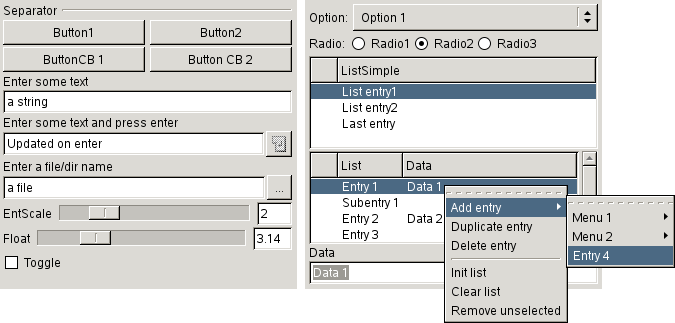
\includegraphics[width=12cm]{iw_widgets}
  \end{center}
  \caption[Die Widgets von \icewing{}]
  {Alle Widgets, die \icewing{} f"ur die Oberfl"achengenerierung zur
    Verf"ugung stellt.}
  \label{fig:p_widgets}
\end{figure}

\paragraph{Graphisches Benutzerinterface}\hfill\\

Widgets lassen sich in \icewing{} auf beliebig vielen Seiten im
\icewing-Hauptfenster, im Kontextmen"u von Anzeigefenstern und im
``Settings''-Fenster von Anzeigefenstern erstellen. In der
Abbildung~\ref{fig:p_icewing} sind diese verschiedenen Stellen zu
sehen. Eine neue Seite im \icewing-Hauptfenster kann mittels der
Funktion
\begin{small}
\linespread{0.9}
\begin{verbatim}
    int opts_page_append (char *title);
\end{verbatim}
\fktindex{opts$\_$page$\_$append()}
\end{small}
erstellt werden. \var{title} gibt den Namen an, der in der Liste
``Categories'' angezeigt wird. Zur"uck gegeben wird ein Index, der
bei der Erstellung von Widgets angegeben werden mu"s. Den Index der
``Settings''-Fenster von Anzeigefenstern, der das Erstellen von
Widgets in diesen Fenstern erlaubt, erh"alt man durch die Funktion
\begin{small}
\linespread{0.9}
\begin{verbatim}
    int prev_get_page (prevBuffer *b);
\end{verbatim}
\fktindex{prev$\_$get$\_$page()}
\end{small}

Widgets lassen sich mit Funktionen erstellen, die jeweils nach dem
Schema \fkt{opts\_<widgetname>\_create()} benannt sind. F"ur vier
verschiedene Widgettypen sind dies beispielsweise
\begin{small}
\linespread{0.9}
\begin{verbatim}
    void opts_separator_create (long page, char *title);
    void opts_button_create (long page, char *title, char *ttip, gint *value);
    void opts_entscale_create (long page, char *title, char *ttip,
                               gint *value, gint left, gint right);
    void opts_float_create (long page, char *title, char *ttip,
                            gfloat *value, gfloat left, gfloat right);
\end{verbatim}
\fktindex{opts$\_$widgetname$\_$create()}
\end{small}
Die Parameterliste der Funktionen ist jeweils einheitlich
aufgebaut. \var{page} gibt an, auf welcher Seite das Widget
erscheinen soll. Neue Widgets werden jeweils unten auf der
angegebenen Seite angef"ugt. \var{title} gibt den Namen des Widgets
an. In Abbildung~\ref{fig:p_widgets} war er beispielsweise
\verb|"Enter some text"| f"ur das String Widget und
\verb|"EntScale"| f"ur den Integer-Slider. Dieser Name mu"s in
Verbindung mit dem Seitennamen programmweit eindeutig sein, da er
auch als Identifier f"ur das Widget eingesetzt wird. Der Identifier
ist dabei \verb|"pagetitle.widgettitle"|. Durch diesen Identifier
l"a"st sich das Widget auch nachtr"aglich ansprechen. \var{ttip}
spezifiziert den Tooltip des Widgets. Durch \var{value} wird die
Adresse einer Variablen angegeben. Die Variable wird von \icewing{}
in einem eigenen Thread im Hintergrund modifiziert, ohne da"s das
Plugin eingreifen mu"s. Die restlichen Parameter spezifizieren
jeweils die erlaubten Werte der Variablen.

Zus"atzlich ist es m"oglich, den Wert eines Widgets nachtr"aglich zu
setzen und ein Widget wieder zu l"oschen. Daf"ur dienen folgende
zwei Funktionen:
\begin{small}
\linespread{0.9}
\begin{verbatim}
    long opts_value_set (char *title, void *value);
    gboolean opts_widget_remove (char *title);
\end{verbatim}
\fktindex{opts$\_$widget$\_$remove()}
\fktindex{opts$\_$value$\_$set()}
\end{small}
\var{title} ist dabei der Identifier eines Widgets. In \var{value}
wird, im Falle eines Integers, der zu setzende Wert
"ubergeben. Ansonsten ist es ein Zeiger auf den zu setzenden
Wert. Soll beispielsweise das Widget \verb|"EntScale"| aus
Abbildung~\ref{fig:p_widgets} auf der Seite \verb|"demo"| auf den
Wert 3 gesetzt werden, kann dies durch
\begin{small}
\linespread{0.9}
\begin{verbatim}
    opts_value_set ("demo.EntScale", GINT_TO_POINTER(3));
\end{verbatim}
\end{small}
geschehen. Beim Setzen des Widget \verb|"Float"| geschieht dies
hingegen durch
\begin{small}
\linespread{0.9}
\begin{verbatim}
    float newval = 3.0;
    opts_value_set ("demo.Float", &newval);
\end{verbatim}
\end{small}

\paragraph{Nichtgraphisches Interface}\hfill\\

In diese automatische Behandlung von Variablen zum Laden und
Speichern lassen sich auch Variablen einf"ugen, denen kein Widget
zugeordnet ist. Dies wird durch die Funktionen
\begin{small}
\linespread{0.9}
\begin{verbatim}
    typedef enum {
        OPTS_BOOL, OPTS_INT, OPTS_LONG, OPTS_FLOAT, OPTS_DOUBLE, OPTS_STRING
    } optsType;

    typedef void (*optsSetFunc) (void *value, void *new_value, void *data);

    void opts_variable_add (char *title, optsSetFunc setval, void *data,
                            optsType type, void *value);
    void opts_varstring_add (char *title, optsSetFunc setval, void *data,
                             void *value, int length);
\end{verbatim}
\fktindex{opts$\_$variable$\_$add()}
\end{small}
erm"oglicht. \var{title} entspricht der \var{titel}-Variablen der
Widget-Funktionen. \var{value} gibt die Adresse der zu
ladenden/speichernden Variablen an. Durch \var{type} wird deren Typ
bekanntgegeben. Ist \var{func} auf \var{NULL} gesetzt, wird die
Variable nicht nur automatisch im Hintergrund gespeichert, sondern
auch geladen und gesetzt. Ansonsten wird, sobald die Variable
modifiziert werden soll, die Funktion \var{setval} mit \var{data}
als einem zus"atzlichen Argument aufgerufen. Diese Funktion ist dann
f"ur das Modifizieren der Variablen verantwortlich. Durch die
Benutzung von \fkt{opts\_varstring\_add()} kann f"ur Strings
zus"atzlich eine Maximall"ange des Strings angegeben werden, die
beim Setzen des Strings nicht "uberschritten wird.

\paragraph{Plugin-Support}\hfill\\

Gewisse durch Widgets steuerbare standardisierte Funktionen sind f"ur
viele Plugins interessant. Zus"atzlich ben"otigen die meisten
Plugins mindestens eine Seite, um dort Widgets zu plazieren. Um dies
zu vereinfachen, gibt es folgende Funktion, die eine neue Seite mit
zwei speziellen Widgets anlegt:
\begin{small}
\linespread{0.9}
\begin{verbatim}
    typedef enum {
        PLUG_PAGE_NOPLUG        = 1 << 0
    } plugPageFlags;

    int plug_add_default_page (plugDefinition *plugDef, char *suffix,
                               plugPageFlags flags);
\end{verbatim}
\fktindex{plug$\_$add$\_$default$\_$page()}
\end{small}
Die Funktion legt eine neue Seite im \icewing{}-Hauptfenster unter
dem Namen '\var{plugDef->name}\verb|" "|\var{suffix}' an und gibt deren
Index zur"uck. Zus"atzlich werden bis zu zwei Widgets angelegt, deren
Funktionalit"at vollst"andig von \icewing{} realisiert wird. Das
erste Widget erm"oglicht das Aktivieren/Deaktivieren des Aufrufs der
\fkt{process()} Funktion des Plugins.

Das zweite Widget wird angelegt, falls nicht
\type{PLUG\_PAGE\_NOPLUG} in \var{flags} angegeben wurde. "Uber
dieses zweite Widget kann gesteuert werden, welche Daten von welchen
anderen Plugins an das Plugin \var{plugDef} weitergereicht werden
sollen. Normalerweise wird die Funktion \fkt{process()} des Plugins
\var{plugDef} aufgerufen, sobald Daten eines Identifiers von einem
beliebigen Plugin vorhanden sind, die von dem Plugin \var{plugDef}
beobachtet werden. Stehen zu diesem Zeitpunkt mehrere Daten des
Identifiers zur Verf"ugung, wird das Plugin trotzdem nur einmal
aufgerufen. Das Plugin kann die zus"atzlichen Daten durch
\fkt{plug\_data\_get()} abrufen.

Durch den Aufruf von \fkt{plug\_add\_default\_page()} wird dieses
Verhalten ge"andert. Ist in diesem Fall im zweiten Widget nichts
eingetragen, wird das Plugin f"ur alle Daten von allen Plugins, f"ur
das sich das Plugin angemeldet hat, getrennt aufgerufen. Werden im
Widget Namen von Plugins eingetragen, wird das Plugin nur f"ur diese
Plugins aufgerufen. Stehen Daten von anderen Plugins zur Verf"ugung,
wird das Plugin nicht aufgerufen.

Da \icewing{} mit diesem Widget zus"atzlich weitere Informationen
"uber die Abh"angigkeiten der Plugins hat, wird hier gegebenenfalls
eine Umsortierung der Aufrufreihenfolge durchgef"uhrt. Beobachten
mehrere Plugins den gleichen Identifier \verb|"ident"|, ist
normalerweise deren Aufrufreihenfolge nicht spezifiziert. Wird in
diesem zweiten Widget aber nun spezifiziert, da"s ein Plugin
\verb|"ident"| von einem dieser anderen Plugins haben m"ochte, wird
sichergestellt, da"s erst dieses andere Plugin aufgerufen wird.

\subsection{Graphische Anzeige von Daten}
\label{sub:p_rendering}

\icewing{} enth"alt verschiedene M"oglichkeiten, Daten zu
visualisieren. Plugins k"onnen beliebig viele Fenster zur
Darstellung von Daten anlegen. Der Benutzer kann diese jederzeit
"offnen oder wieder schlie"sen, in ihnen zoomen und scrollen, ihren
Inhalt abspeichern oder sich Metainformationen "uber den Inhalt
anzeigen lassen. Bei all diesen Aktionen sind die Plugins nicht
involviert. Um die n"otigen Zoom- und Redrawaktionen k"ummert sich
vollst"andig \icewing{}. Vektorobjekte wie Linien und Ellipsen
werden dabei je nach Zoomstufe neu gezeichnet.

\paragraph{Verwaltung von Fenstern}\hfill\\

Neue Fenster k"onnen mit der Funktion
\begin{small}
\linespread{0.9}
\begin{verbatim}
    typedef struct prevBuffer {
        ...
        guchar *buffer;         /* Buffer fuer das zu erzeugende Bild */
        int width, height;      /* Breite, Hoehe des Buffers */
        GtkWidget *window;      /* Fenster fuer den Buffer */
        ...
    } prevBuffer;

    prevBuffer *prev_new_window (char *title, int width, int height,
                                 gboolean gray, gboolean show);
\end{verbatim}
\typeindex{prevBuffer}
\fktindex{prev$\_$new$\_$window()}
\end{small}
angelegt werden. \var{title} ist einerseits der Name des Fensters
und andererseits ein Identifier, der zusammen mit den Namen der mit
\fkt{opts\_page\_append()} angelegten Seiten im
\icewing-Hauptfenster programmweit eindeutig sein mu"s. Enth"alt der
Name einen Punkt (\verb|"."|), werden die Fenster in der
``Images''-Liste im Hauptfenster in einer Baumstruktur
angezeigt. \var{width} und \var{height} geben die initiale Gr"o"se
des Fensters an. Der Benutzer kann die Fenstergr"o"se nachtr"aglich
jederzeit "andern. Durch Angabe von \var{-1} wird die Standardbreite
beziehungsweise H"ohe genommen. \var{gray} gibt an, ob alles in
Graustufen oder in Farbe dargestellt werden soll. Durch \var{show =
TRUE} wird das Fenster immer nach dem Anlegen sofort
ge"offnet. Ansonsten passiert dies erst, wenn der Benutzer das
Fenster per Doppelklick in der ``Images''-Liste "offnet.

Nennenswert Speicher wird durch ein Fenster erst nach dem ersten
"Offnen verbraucht. Alle \icewing-Funktionen zum Zeichnen in einem
Fenster testen zuerst, ob es offen ist und kehren sofort zur"uck,
falls dies nicht der Fall ist. Damit ist es aus der Sicht des
Ressourcenverbrauchs unproblematisch, viele Fenster anzulegen und
Ausgaben in diesen ohne weitere Tests vorzunehmen. Sind Berechnungen
f"ur die Ausgabe von Daten n"otig, kann ein Test, ob ein Fenster
offen ist, aber sinnvoll sein. Dies kann durch
\verb|(buffer->window != NULL)| geschehen. Durch
\begin{small}
\linespread{0.9}
\begin{verbatim}
    void prev_free_window (prevBuffer *b);
\end{verbatim}
\fktindex{prev$\_$free$\_$window()}
\end{small}
kann ein per \fkt{prev\_new\_window()} angelegtes Fenster
schlie"slich wieder entfernt werden.

Der Benutzer kann in den Fenstern jederzeit zoomen und
scrollen. Zus"atzlich k"onnen diese Aktionen auch programmgesteuert
durch die Funktion
\begin{small}
\linespread{0.9}
\begin{verbatim}
    void prev_pan_zoom (prevBuffer *b, int x, int y, float zoom);
\end{verbatim}
\fktindex{prev$\_$pan$\_$zoom()}
\end{small}
durchgef"uhrt werden. Der Inhalt des Fenster \var{b} wird an der
Stelle \var{(x,y)} mit einem Zoom-Wert von \var{zoom}
dargestellt. Sind einzelne Werte kleiner Null, werden die
entsprechenden alten Werte nicht ver"andert.

Zum Teil ist es n"otig, da"s ein Plugin Informationen "uber
Mausaktionen und Tastendr"ucke in einem Fenster bekommt. Dies wird
durch die Funktionen
\begin{small}
\linespread{0.9}
\begin{verbatim}

    typedef enum {
        PREV_BUTTON_PRESS               = 1 << 0,
        PREV_BUTTON_RELEASE             = 1 << 1,
        PREV_BUTTON_MOTION              = 1 << 2
        PREV_KEY_PRESS                  = 1 << 3,
        PREV_KEY_RELEASE                = 1 << 4
    } prevEvent;
    typedef void (*prevButtonFunc) (prevBuffer *b, prevEvent signal,
                                    int x, int y, void *data);
    typedef void (*prevSignalFunc) (prevBuffer *b, prevEventData *event,
                                    void *data);

    void prev_signal_connect (prevBuffer *b, prevEvent sigset,
                              prevButtonFunc cback, void *data);
    void prev_signal_connect2 (prevBuffer *b, prevEvent sigset,
                               prevSignalFunc cback, void *data);
\end{verbatim}
\fktindex{prev$\_$signal$\_$connect()}
\fktindex{prev$\_$signal$\_$connect2()}
\end{small}
erm"oglicht. Tritt eins der mittels \var{sigset} angegebenen
Ereignisse ausgel"ost mit der linken Maustaste oder einer Taste im
Fenster \var{b} auf, wird die Funktion \fkt{cback()} mit \var{data}
als zus"atzliches Argument aufgerufen. \fkt{cback()} wird
zus"atzlich mit dem aufgetretenem Signal und weiteren Informationen
"uber das Ereignis aufgerufen. \fkt{prev\_signal\_connect()} erlaubt
dabei nur die Verarbeitung von Mausereignissen,
\fkt{prev\_signal\_connect2()} sowohl Maus- als auch
Tastaturereignisse. Bei allen Mauskoordinaten sind jeweils
Modifikationen durch Zoomen und Scrollen herausgerechnet. 

\paragraph{Darstellung von graphischen Objekten}\hfill\\

\begin{figure}[htb]
  \begin{center}
    \includegraphics[width=\textwidth]{iw_render}
  \end{center}
  \caption[Die graphischen Elemente von \icewing{}]
  {Alle graphischen Elemente, die \icewing{} darstellen kann.}
  \label{fig:p_render}
\end{figure}

\icewing{} bietet die M"oglichkeit, verschiedene Graphikprimitiva in
den Fenstern darzustellen. Abbildung~\ref{fig:p_render} zeigt eine
"Ubersicht aller in \icewing{} enthaltener Objekte. Die Darstellung
der Objekte ist mehrstufig. In einem ersten optionalen Schritt wird
eine Kopie aller Originaldaten angelegt, die f"ur die Darstellung
eines Objektes ben"otigt werden. Damit erh"alt \icewing{} die
M"oglichkeit, das Bild komplett ohne Interaktion mit dem Plugin neu
aufzubauen -- Scrollen und Zoomen ohne Pluginhilfe wird m"oglich.
Anschlie"send werden die Objekte entsprechend den aktuellen Scroll-
und Zoomwerten in einem Offscreenbuffer dargestellt. Dieser Buffer
zeigt exakt den Bildausschnitt, der auch im Fenster zu sehen sein
wird, und kann damit f"ur ein Redraw des Fensters eingesetzt
werden -- wiederum ohne Interaktion mit dem Plugin. In einem finalen
Schritt wird der Buffer schlie"slich in das Fenster "ubertragen.

Die verschiedenen Objekte k"onnen "uber ein einheitliches Interface
verschiedener Funktionen dargestellt werden. Zwei von ihnen sind
\begin{small}
\linespread{0.9}
\begin{verbatim}
    typedef enum {
        PREV_IMAGE,
        PREV_TEXT,
        PREV_LINE,
        ...
        PREV_NEW = 30
    } prevType;

    #define RENDER_THICK    (1<<30)  /* beachte die thickness-Einstellung */
    #define RENDER_CLEAR    (1<<31)  /* loesche den Buffer */

    void prev_render_data (prevBuffer *b, prevType type, void *data,
                           int disp_mode, int width, int height);
    void prev_render_list (prevBuffer *b, prevType type, void *data,
                           int size, int cnt,
                           int disp_mode, int width, int height);
\end{verbatim}
\typeindex{prevType}
\fktindex{prev$\_$render$\_$data()}
\fktindex{prev$\_$render$\_$list()}
\end{small}
Bei allen Renderfunktionen gibt es verschiedene
Standardargumente. In dem Fenster \var{b} wird das Objekt
dargestellt. \var{width} und \var{height} geben die Gesamtgr"o"se
aller Objekte an, die in dem Fenster noch dargestellt werden. Diese
beiden Werte werden ben"otigt, um gegebenenfalls den Zoomfaktor f"ur
die Darstellung des Objektes korrekt zu berechnen, falls ein ``Fit
to window''-Darstellungsmodus f"ur das Fenster gew"ahlt ist. "Uber
\var{disp\_mode} kann die Darstellungsart modifiziert werden. Das
Flag \var{RENDER\_CLEAR} l"oscht vor dem Zeichnen sowohl den Inhalt
des kompletten Fensters als auch die internen Kopien aller Parameter
aller vorher durchgef"uhrten Zeichenaktionen. \var{RENDER\_THICK}
erlaubt die dickere Darstellung von Linien entsprechend einer
gesondert gew"ahlten Einstellung. Die restlichen Argumente
spezifizieren jeweils das darzustellende Objekt. Bei
\fkt{prev\_render\_data()} wird ein beliebiges Objekt dargestellt,
bei \fkt{prev\_render\_list()} ein Feld gleicher Objekte. \var{type}
gibt den Typ der Objekte an. \var{data} ist entweder ein Zeiger auf
die Daten eines Objektes oder ein Zeiger auf ein Feld von
Objektdaten. Im zweiten Fall wird "uber \var{cnt} die L"ange des
Feldes und "uber \var{size} die Gr"o"se eines Feldelementes
angegeben.

Werte f"ur darzustellende Objekte werden "uber Strukturen
angegeben. F"ur Linien ist dies beispielsweise
\begin{small}
\linespread{0.9}
\begin{verbatim}
    typedef struct {
        iwColtab ctab;
        int r, g, b;
        int x1, y1, x2, y2;
    } prevDataLine;
\end{verbatim}
\typeindex{prevDataLine}
\end{small}
Die Strukturen der restlichen vorhandenen Objekte sind vergleichbar
aufgebaut. "Uber \var{ctab} wird angegeben, wie \var{r}, \var{g} und
\var{b} interpretiert werden sollen. Durch das Setzen von \var{ctab}
auf \var{IW\_RGB} werden sie beispielsweise als Punkt im
RGB-Farbraum interpretiert, durch \var{IW\_YUV} als Punkt im
YUV-Farbraum und durch einen Zeiger auf eine Farbtabelle wird
\var{r} als Index in diese Farbtabelle interpretiert. Die Angabe von
\var{-1} f"ur \var{r}, \var{g} oder \var{b} hat eine
Sonderbedeutung. In diesem Fall wird der entsprechende Farbkanal
beim Darstellen des Objektes nicht ge"andert. \var{x1}, \var{y1},
\var{x2} und \var{y2} sind schlie"slich die Koordinaten der
Endpunkte der Linie. Um ein subpixelgenaues Darstellen von Objekten
zu erm"oglichen, gibt es von den Strukturen f"ur Vektorobjekte
jeweils Varianten mit \var{float}-Datentypen, beispielsweise
\typeIndex{prevDataLineF} f"ur Linien. Zur Darstellung gibt es
entsprechende \type{prevType}-Werte, f"ur Linien beispielsweise
\var{PREV\_LINE\_F}.

Um den Aufruf zu vereinfachen gibt es f"ur
\fkt{prev\_render\_list()} je einen Wrapper pro Objekttyp. Felder
von Linien oder Bildern lassen sich beispielsweise auch durch
\begin{small}
\linespread{0.9}
\begin{verbatim}
    void prev_render_lines (prevBuffer *b, prevDataLine *lines, int cnt,
                            int disp_mode, int width, int height);
    void prev_render_imgs (prevBuffer *b, prevDataImage *imgs, int cnt,
                           int disp_mode, int width, int height);
\end{verbatim}
\fktindex{prev$\_$render$\_$lines()}
\fktindex{prev$\_$render$\_$imgs()}
\end{small}
darstellen. Bei der Bildverarbeitung mu"s sehr h"aufig ein Bild
dargestellt werden. F"ur den h"aufigen Fall von 8 Bit Bildern gibt
es daf"ur 
\begin{small}
\linespread{0.9}
\begin{verbatim}
    void prev_render (prevBuffer *b, guchar **planes,
                      int width, int height, iwColtab ctab);
\end{verbatim}
\fktindex{prev$\_$render()}
\end{small}
womit in diesem Fall keine Struktur gef"ullt werden mu"s. Diese
Funktion l"oscht zus"atzlich durch Setzen von \var{RENDER\_CLEAR}
vor der Darstellung des Bildes das komplette Fenster. Sollen andere
Bildtypen dargestellt werden, \icewing{} unterst"utzt auch
Bildtiefen von 16 Bit, 32 Bit, Float und Double, oder wird
anderweitig mehr Flexibilit"at ben"otigt, m"ussen entweder
\fkt{prev\_render\_imgs()} oder die allgemeinen Renderfunktionen
benutzt werden.

F"ur die vereinfachte Textausgabe gibt es zus"atzlich die Funktion
\begin{small}
\linespread{0.9}
\begin{verbatim}
    void prev_render_text (prevBuffer *b, int disp_mode, int width, int height,
                           int x, int y, char *format, ...);
\end{verbatim}
\fktindex{prev$\_$render$\_$text()}
\end{small}
Diese Funktion f"uhrt intern ein \fkt{sprintf()} aus und gibt den
erhaltenen String dann aus. Im String k"onnen zus"atzlich
Formatierungsanweisungen enthalten sein, um Farbe, Art und
Ausrichtung zu modifizieren. Durch ein eingebettetes
\verb|<fg="255 0 0" bg="0 0 0" font=big>| kann beispielsweise auf
einen gro"sen roten Font auf schwarzem Grund umgestellt werden. Weitere
Details zu den m"oglichen Formatierungsanweisungen finden sich im
Header ``Grender.h''.

Die Darstellung von Objekten l"a"st sich durch zwei weitere
Funktionen beeinflussen:
\begin{small}
\linespread{0.9}
\begin{verbatim}
    void prev_set_bg_color (prevBuffer *buf, uchar r, uchar g, uchar b);
    void prev_set_thickness (prevBuffer *buf, int thickness);
\end{verbatim}
\fktindex{prev$\_$set$\_$bg$\_$color()}
\fktindex{prev$\_$set$\_$thickness()}
\end{small}
\fkt{prev\_set\_bg\_color()} gibt an, mit welcher Farbe das Fenster
bei Auftreten von \var{RENDER\_CLEAR} gel"oscht werden soll. Durch
\fkt{prev\_set\_thickness()} werden Linien in der angegebenen Dicke
gezeichnet, falls \var{RENDER\_THICK} bei der Ausgabe von Objekten
mit angegeben war.

Alle bisher beschriebenen Funktionen zum Darstellen von Objekten
zeichnen die Objekte inkrementell in einen einem Fenster
zugeordneten Offscreenbuffer. Dieser l"a"st sich in einem finalen
Schritt mittels
\begin{small}
\linespread{0.9}
\fktindex{prev$\_$draw$\_$buffer()}
\begin{verbatim}
    void prev_draw_buffer (prevBuffer *b);
\end{verbatim}
\end{small}
in dem Fenster darstellen. Zusammenfassend sind somit folgende
Schritte n"otig, um mittels \icewing{} etwas in einem Fenster
darzustellen:
\begin{equation*}
  \parbox{14.5cm}{\begin{struktogramm}{14.5cm}{0.4cm}
    \BLOCK{Anlegen eines neuen Fensters \var{b} mittels
      \fkt{prev\_new\_window()}. Dies ist initial einmal n"otig. Eine
      gute Stelle hierf"ur ist die Funktion \fkt{init\_options()} des
      Plugins.}
    \LOOP{
      \BLOCK{Darstellen beliebiger Objekte in dem Offscreenbuffer des
        Fensters \var{b} durch mehrfaches Aufrufen von
        \fkt{prev\_render\_xxx()}-Funktionen. Bei dem ersten Aufruf
        sollte \var{RENDER\_CLEAR} gesetzt sein, um das Fenster zu
        l"oschen.}
      \BLOCK{Darstellen des Offscreenbuffers im Fenster \var{b} durch
        Aufruf der Funktion \fkt{prev\_draw\_buffer()}.}
    }
  \end{struktogramm}}
\end{equation*}
Neben diesem hier beschriebenen Interface mit den
\fkt{prev\_render\_xxx()}-Funktionen zur Darstellung von Objekten
gibt es auch noch ein Interface bestehend aus
\fkt{prev\_drawXxx()}-Funktionen. Dies ist ein Interface niedriger
Abstraktionsrate, welches beispielsweise die Scrollposition oder die
Zoomeinstellung ignoriert. Weitere Details hierzu finden sich in den
entsprechenden Headern.

\subsection{Weitere graphische Funktionalit"aten}

Mu"s die Programmausf"uhrung beendet werden, sollte dies niemals mit
der normalen ANSI-Funktion \fkt{exit()} geschehen. F"ur das
sofortige Beenden des Programms sollte immer die Funktion
\begin{small}
\linespread{0.9}
\begin{verbatim}
    void gui_exit (int status);
\end{verbatim}
\fktindex{gui$\_$exit()}
\end{small}
benutzt werden. Der direkte Aufruf von \fkt{exit()} kann sowohl zu
einer ``Segmentation violation'' als auch zum Stehenbleiben des
Programms f"uhren. Da verschiedene graphische Funktionalit"aten mit
Hilfe eines eigenen Threads realisiert sind, mu"s beim Beenden eine
korrekte Synchronisierung mit diesem Thread
stattfinden. \fkt{gui\_exit()} stellt dies sicher.

Bilder werden in \icewing{} durch die Struktur
\begin{small}
\linespread{0.9}
\begin{verbatim}
    typedef enum {
        IW_8U, IW_16U, IW_32S, IW_FLOAT, IW_DOUBLE
    } iwType;

    typedef struct iwImage {
        guchar *data[3];    /* Die eigentlichen Bilddaten */
        int planes;         /* Anzahl der Farbebenen von data */
        iwType type;        /* Typ von data */
        int width, height;  /* Breite, Hoehe des Bildes in Pixel */
        int rowstride;      /* Abstand zweier Linien in Bytes */
                            /*   >0: Farbbilder sind interleaved in data[0] */
        iwColtab ctab;      /* Farbraum von data */
    } iwImage;
\end{verbatim}
\typeindex{iwType}
\typeindex{iwImage}
\end{small}
verwaltet. Die Bilddaten k"onnen hier in verschiedenen Typen und in
verschiedenen Anordnungen abgelegt sein. Durch \type{iwType} wird
der Typ von \var{data} spezifiziert -- von 8 Bit unsigned bis
double. Die Anordnung der Daten kann sowohl \emph{planed} als auch
\emph{interleaved} sein. Bei einer planed Anordnung sind die
einzelnen Farbebenen des Bildes getrennt voneinander in
\var{data[0]}, \var{data[1]} und \var{data[2]} angegeben. Bei
interleaved enth"alt \var{data[0]} die einzelnen Farbwerte f"ur
jedes Pixel direkt hintereinander. F"ur \var{planes=3} im
RGB-Farbraum kommt beispielsweise zuerst der Rotwert von Pixel 1,
dann der Gr"unwert und der Blauwert. Anschlie"send kommen diese drei
Werte f"ur Pixel 2 bis schlie"slich die drei Werte f"ur Pixel
\var{width*heigth} in \var{data[0]} abgelegt sind. Bilder aller
dieser Typen und Anordnungen k"onnen sowohl angelegt, freigegeben,
geladen, gespeichert als auch angezeigt werden.

F"ur die Verwaltung von Bildern gibt es verschiedene
Funktionen. Einige wichtige sind
\begin{small}
\linespread{0.9}
\begin{verbatim}
    iwImage* iw_img_new (void);
    iwImage* iw_img_new_alloc (int width, int height, int planes, iwType type);
    void     iw_img_free (iwImage *img, iwImgFree what);
    iwImage* iw_img_load (char *fname, iwImgStatus *status);
    iwImgStatus iw_img_save_format (iwImage *img, iwImgFormat format,
                                    char *fname, iwImgFileData *data);
\end{verbatim}
\fktindex{iw$\_$img$\_$new()}
\fktindex{iw$\_$img$\_$new$\_$alloc()}
\fktindex{iw$\_$img$\_$free()}
\fktindex{iw$\_$img$\_$load()}
\fktindex{iw$\_$img$\_$save$\_$format()}
\end{small}
Weitere Details zu diesen Funktionen sowie verschiedene andere
Funktionen zur Verwaltung von Bildern finden sich im Header
``Gimage.h''.

\section{Weitere Funktionalit"aten}

Neben den bisher beschriebenen Funktionalit"aten stehen weitere
sowohl im graphischen Bereich als in anderen Bereichen zur
Verf"ugung. In diesem Abschnitt wird eine Auswahl von ihnen n"aher
vorgestellt. Daneben gibt es andere, die nicht genauer vorgestellt
werden. Im Header ``output.h'' finden sich beispielsweise
Funktionen zur Vereinfachung der Ausgabe von Daten "uber \dacs{}. Es
stehen Funktionen zur Ausgabe von Bildern, zur Ausgabe von
Statusmeldungen und zur Ausgabe von allgemeinen Daten "uber Streams
zur Verf"ugung. Weiterhin k"onnen Funktionen "uber \dacs{} zur
Verf"ugung gestellt werden. Die Anmeldung bei \dacs{}, die
Fehlerbehandlung und die Generierung eindeutiger Stream- und
Funktionsnamen werden jeweils von diesen Funktionen "ubernommen.

Weitere Beispiele f"ur weitere Funktionen sind das ``session
management'' oder Funktionen f"ur das Registrieren eines neuen
Graphikprimitives, um diesen mit den allgemeinen Renderfunktionen
darzustellen. Weitere Details zu diesen wie auch zu den bisher
vorgestellten Funktionen finden sich in den verschiedenen Headern
von \icewing{}.

\paragraph{Das Plugin ``grab''}\hfill\\
\index{grab}

Ein zentrales Plugin ist das in \icewing{} eingebaute Plugin
``grab''. Es erm"oglicht das Einlesen und Weiterreichen einer Folge
von Bildern. Die Bilder k"onnen von einem Grabber (angesteuert durch
Video4Linux 2 oder FireWire unter Linux und MME auf Alphas), von
\dacs{} im \type{Bild\_t}-Format oder aus Dateien verschiedener
Pixelformate eingelesen werden. Sobald das Plugin von \icewing{}
aufgerufen wird, liest es das n"achste Bild ein und stellt es mit
Hilfe von \fkt{plug\_data\_set()} unter dem Ident \verb|"image"|
f"ur andere Plugins zur Verf"ugung. Als Format wird dabei das
folgende \type{grabImageData} benutzt:
\begin{small}
\linespread{0.9}
\begin{verbatim}
    typedef struct grabImageData {
        iwImage *img;         /* Das eigentliche Bild */
        struct timeval time;  /* Zeitpunkt des Grabbens */
        int img_number;       /* Fortlaufende Nummer */
        char *fname;          /* Bild aus einer Datei? -> Name der Datei */
        int downw, downh;     /* Faktor, um den das Bild verkleinert wurde */
    } grabImageData;
\end{verbatim}
\typeindex{grabImageData}
\end{small}
Zus"atzlich stellt es die eingelesenen Bilder wahlweise auch "uber
einen \dacs-Stream im \type{Bild\_t}-Format zur Verf"ugung. "Uber
eine \dacs-Funktion k"onnen das aktuelle und wahlweise auch "altere
Bilder ebenfalls im \type{Bild\_t}-Format von anderen Programmen
abgeholt werden. Existiert ein Observer f"ur den Ident
\verb|"imageRGB"|, wird das aktuelle Bild zus"atzlich mit Hilfe von
\fkt{plug\_data\_set()} unter diesem Ident im RGB-Farbraum zur
Verf"ugung gestellt. Dazu wird wiederum der Typ \type{grabImageData}
benutzt.

\paragraph{Hilfsfunktionen}\hfill\\

``tools.h'' stellt verschiedene kleinere Hilfsroutinen zur
Verf"ugung, die immer wieder ben"otigt werden. Dazu geh"oren
Funktionen zur Ausgabe von Fehlern, von Warnungen, von
Debugmeldungen und Funktionen zum Testen von Assertions:
\begin{small}
\linespread{0.9}
\begin{verbatim}
    void iw_debug (int level, char *str, ...);
    void iw_debug_1 (int level, char *str);
    void iw_debug_2 (int level, char *str, ARG1);
    ...
    void iw_warning (char *str, ...);
    void iw_warning_1 (char *str);
    void iw_warning_2 (char *str, ARG1);
    ...
    void iw_error (char *str, ...);
    void iw_error_1 (char *str);
    void iw_error_2 (char *str, ARG1);
    ...
    void iw_assert (scalar expression, char *str, ...);
    void iw_assert_1 (scalar expression, char *str);
    void iw_assert_2 (scalar expression, char *str, ARG1);
    ...
\end{verbatim}
\end{small}
Alle diese Funktionen f"uhren intern ein \fkt{sprintf()} aus. Die
Funktionen \fktIndex{iw$\_$debug$\_$xxx()} und \fktIndex{iw$\_$assert$\_$xxx()}
erzeugen nur dann Code, wenn das Macro \var{DEBUG} beim Kompilieren
gesetzt ist. \fkt{iw\_debug$\_$xxx()} gibt nur dann etwas aus, wenn
\var{level} kleiner als der "uber die \icewing-Kommandozeile
gew"ahlte \var{talklevel} ist. \fktIndex{iw$\_$warning$\_$xxx()} gibt die
Meldung immer aus, \fktIndex{iw$\_$error$\_$xxx()} bricht zus"atzlich die
Programmausf"uhrung ab. Die Varianten ohne eine Zahl im Namen, d.h
\fkt{iw\_debug()}, \fkt{iw\_warning()}, \fkt{iw\_error()} und
\fkt{iw\_assert()}, erlauben eine beliebige Anzahl von
Argumenten. Sie ben"otigen allerdings f"ur die vollst"andige
Funktion entweder den GCC oder einen ANSI-C99 kompatiblen
Compiler. Ansonsten sind diese Varianten nicht als Macro, sondern
als Funktionen realisiert, die weniger Informationen als die
Macro-Varianten zur Verf"ugung stellen.

Auch f"ur die Messung der Ausf"uhrungszeit von Programmteilen stehen
verschiedene Funktionen zur Verf"ugung. Unter anderem sind dies
\begin{small}
\linespread{0.9}
\begin{verbatim}
    int  iw_time_add (char *name);
    void iw_time_start (int nr);
    long iw_time_stop (int nr, BOOL show);

    #define iw_time_add_static(number,name) ...
    #define iw_time_add_static2(number,name,number2,name2) ...
\end{verbatim}
\fktindex{iw$\_$time$\_$add()}
\fktindex{iw$\_$time$\_$start()}
\fktindex{iw$\_$time$\_$stop()}
\fktindex{iw$\_$time$\_$add$\_$static()}
\end{small}
\fkt{iw\_time\_add()} legt einen neuen Zeitmesser an und gibt einen
Index zum Ansprechen des Messers zur"uck. Per
\fkt{iw\_time\_start()} kann er gestartet und per
\fkt{iw\_time\_stop()} wieder gestoppt werden. Durch \var{show =
TRUE} wird die vergangene Zeit direkt nach \var{stdout}
ausgegeben. Ansonsten geschieht dies nach einer gewissen Anzahl
Durchl"aufe der Hauptschleife. "Uber \fkt{iw\_time\_add\_static()}
kann die Initialisierung vereinfacht werden. Hier wird eine neue
static Variable mit Namen \var{number} definiert und per einmaligem
Aufruf von \fkt{iw\_time\_add()} initialisiert. Die Benutzung kann
wie folgt aussehen:
\begin{small}
\linespread{0.9}
\begin{verbatim}
    /* Definition anderer Variablen */
    ...
    iw_time_add_static (time_demo, "Demo Messung");

    iw_time_start (time_demo);
    /* Ausfuehrung des zu messenden Programmteils */
    ...
    iw_time_stop (time_demo, FALSE);
\end{verbatim}
\end{small}

Die Auswertung von Kommandozeilenargumenten wird durch die Funktion
\begin{small}
\linespread{0.9}
\begin{verbatim}
  char iw_parse_args (int argc, char **argv, int *nr, void **arg, char *pattern);
\end{verbatim}
\fktindex{iw$\_$parse$\_$args()}
\end{small}
erleichtert. Die Funktion testet, ob \var{argv[*nr]} in
\var{pattern} vorhanden ist, wobei die Gro"s-/Kleinschreibung von
\var{argv[*nr]} ignoriert wird. Anschlie"send wird \var{*nr} passend
erh"oht, so da"s beim n"achsten Aufruf von \fkt{iw\_parse\_args()}
das n"achste Argument untersucht werden kann. Das Format von
\var{pattern} in EBNF ist
\verb#{ "-" token ":" ch ["r"|"ro"|"i"|"io"|"f"|"fo"|"c"] " " }#,
wobei \var{token} ein beliebiger String ohne \verb|" "| und
\verb|":"| ist und \var{ch} ein beliebiges Zeichen ist. \var{ch}
wird zur"uckgegeben, falls \var{-token} gefunden wurde. Die
restlichen optionalen Zeichen in \var{pattern} sind
Modifikatoren. \verb|"r"| gibt an, da"s zus"atzlich ein Argument
ben"otigt wird, welches in der Variablen \var{arg} zur"uckgegeben
wird. Bei \verb|"i"| wird ein zus"atzliches Integer-Argument
ben"otigt, bei \verb|"f"| ein Float-Argument. \verb|"c"| bedeutet,
da"s \var{token} beliebig fortgesetzt werden kann. Diese Fortsetzung
wird in der Variablen \var{arg} zur"uckgegeben. Durch \verb|"o"|
kann schlie"slich angegeben werden, da"s das String- oder
Int-Argument optional ist. Die Anwendung der Funktion
\fkt{iw\_parse\_args()} zeigt am einfachsten ein Beispiel:
\begin{small}
\linespread{0.9}
\begin{verbatim}
    void *arg;
    char ch, *str_arg;
    int nr = 0, int_arg;

    str_arg = NULL;
    int_arg = 0;
    while (nr < argc) {
        ch = iw_parse_args (argc, argv, &nr, &arg,
                            "-I:Ii -S:Sr -H:H -HELP:H --HELP:H");
        switch (ch) {
            case 'I':
                int_arg = (int)(long)arg;
                break;
            case 'S':
                str_arg = (char*)arg;
                break;
            case 'H':
            case '\0':
                help();
            default:
                fprintf (stderr, "Unknown character %c!\n", ch);
                help();
        }
    }
\end{verbatim}
\end{small}

\selectlanguage{english}

%%% Local Variables: 
%%% mode: latex
%%% TeX-master: "../iceWing"
%%% fill-column: 68
%%% End: 
